% Created 2021-12-20 Mon 20:43
% Intended LaTeX compiler: pdflatex
\documentclass[11pt]{article}
\usepackage[utf8]{inputenc}
\usepackage[T1]{fontenc}
\usepackage{graphicx}
\usepackage{grffile}
\usepackage{longtable}
\usepackage{wrapfig}
\usepackage{rotating}
\usepackage[normalem]{ulem}
\usepackage{amsmath}
\usepackage{textcomp}
\usepackage{amssymb}
\usepackage{capt-of}
\usepackage{hyperref}
\usepackage{minted}
\usepackage{fullpage}
\usepackage{amssymb}
\usepackage[english]{babel}
\usepackage{graphicx,multirow}
\usepackage{caption}
\usepackage{hyperref}
\usepackage{amsmath}
\usepackage{enumitem}
\usepackage{subfig}
\usepackage{placeins}
\captionsetup{font=bf,belowskip=8pt}
\author{stfn}
\date{\today}
\title{}
\hypersetup{
 pdfauthor={stfn},
 pdftitle={},
 pdfkeywords={},
 pdfsubject={},
 pdfcreator={Emacs 27.1 (Org mode 9.5)}, 
 pdflang={English}}
\begin{document}

\begin{document}
\begin{titlepage}
  \newcommand{\HRule}{\rule{\linewidth}{0.5mm}}
  \center
  \textsc{\LARGE Polytechnique Montréal}\\[1.5cm]
  \textsc{\Large LOG8415 : Final Project}\\[0.5cm]
  \textsc{\large Advanced Concepts in Cloud Computing}\\[0.5cm]
  \HRule\\[0.4cm]
          {\huge\bfseries Fully automated web site deployment using S3 static pages}\\[0.4cm]
          \HRule\\[1.5cm]
                  {\large\textit{Authors}}\\
                  Estefan \textsc{Vega-Calcada} (1934346)\\
                  \vfill\vfill\vfill {\large\today} \vfill\vfill
                  
\includegraphics{./images/poly_logo.png}\\[1cm]
                  \vfill
\end{titlepage}

\tableofcontents
\pagebreak

\section{Abstract}
\paragraph{}

When dealing with Big Data, we can choose from a variety of softwares to manage the data sets. A modern, scalable and cost-effective solution is to use software such as Apache Hadoop or Apache Spark to efficiently split the workload across a network of computers (\textit{"nodes"}) and therefore lower the execution time of large tasks. In this paper, we will explore both softwares and compare their differences and evaluate their performances by conducting a few experiments.

\paragraph{Keywords:}Amazon Elastic Compute Cloud, Benchmark, Instance Performance, Cloud Application, MapReduce, Hadoop, Spark, Big Data, AWS
\pagebreak

\section{Introduction} \label{sec:introduction}
\paragraph{} For my final project of the “Advanced Concepts of Cloud Computing” class, I chose to automate the deployment of a simple HTML web page using the various services offered on AWS. In this report, I will explain how I successfully used an S3 bucket and a pipeline to do so. The following is divided into X sections: the issue

\bigskip

\noindent This paper presents some of our experiments with a WordCount program (section ~\ref{sec:WordCount}), the results of our performance comparison between Hadoop and Linux (section ~\ref{sec:HadoopVsLinux}), the results of our performance comparison between Hadoop and Spark (section ~\ref{sec:HadoopVsSpark}) and our solution to the MapReduce program that implements the \textit{People You
  Might Know} social network friendship recommendation algorithm (section ~\ref{sec:MapReduceDescription} and section ~\ref{sec:MapReduceAlgorithm}). All the code presented in this report can be found on our GitHub repository. The link is provided in the Annex (section ~\ref{sec:Annex}).

\section{Experiments with WordCount program} \label{sec:WordCount}

\paragraph{} We implemented our own version of a WordCount program in Java. In the two following sections (section ~\ref{sec:HadoopVsLinux} and ~\ref{sec:HadoopVsSpark}), we present the performances of our program using Linux, Hadoop and Spark. The code we used for our Apache Spark program is inspired from Cloudera's solution \cite{4} and the one we used for our Apache Hadoop program is inspired by the examples from Hadoop's official documentation \cite{5}.

\section{Performance comparison of Hadoop vs Linux} \label{sec:HadoopVsLinux}

\begin{center}
  \captionof{figure}{Comparison between Hadoop and Linux for the 9 texts}
  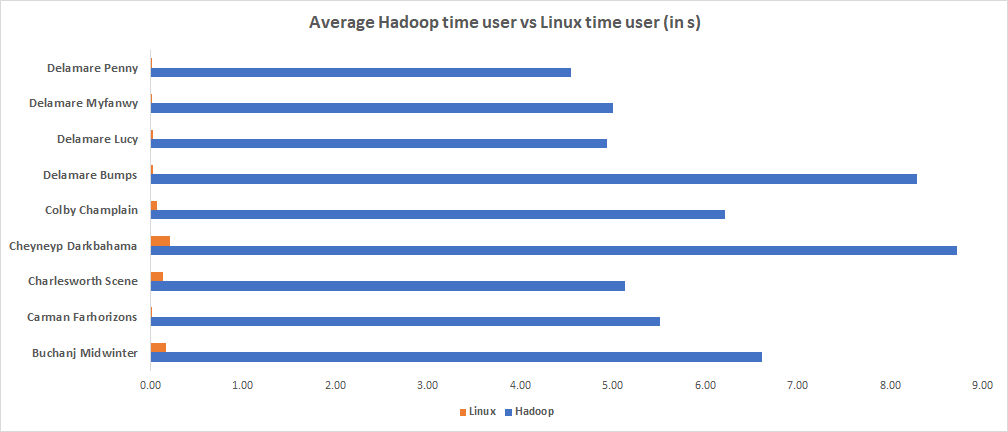
\includegraphics[width=\linewidth]{./images/hadoop-linux.png}
\end{center}

\begin{center}
  \captionof{table}{Comparison between Hadoop and Linux for the 9 texts} \label{tab:regression_analysis_summary}
  \begin{tabular}{|*{3}{c|}}
    \hline
    \textbf{Document} & \textbf{Hadoop time (in s)} & \textbf{Linux time (in s)} \\
    \hline
    buchanj-midwinter-00-t.txt & 6.608 & 0.172 \\
    \hline
    carman-farhorizons-00-t.txt & 5.512 & 0.016 \\
    \hline
    colby-champlain-00-t.txt & 6.216 & 0.076 \\
    \hline
    cheyneyp-darkbahama-00-t.txt & 8.720 & 0.212 \\
    \hline
    delamare-bumps-00-t.txt & 8.288 & 0.028 \\
    \hline
    charlesworth-scene-00-t.txt & 5.136 & 0.132\\
    \hline
    delamare-lucy-00-t.txt & 4.936 & 0.028\\
    \hline
    delamare-myfanwy-00-t.txt & 5.004 & 0.020\\
    \hline
    delamare-penny-00-t.txt & 4.544 & 0.012 \\
    \hline
  \end{tabular}
\end{center}

\subsection{Results}
\paragraph{} The results show that our local Linux machine outperformed Hadoop by alot. This can be explained by the fact Hadoop is meant to process very large data sets. In this scenario, we are dealing with pretty small data sets, that is why our local Linux easily outperformed Hadoop. We would expect Hadoop to perform much better than our local Linux machine if we were dealing with larger data sets, such as the \textit{People You May Know} algorithm ~\ref{sec:MapReduceDescription}.

\section{Performance comparison of Hadoop vs Spark on AWS} \label{sec:HadoopVsSpark}

\paragraph{} For this experimentation, we leveraged AWS EC2 instances. As for the instance type, we used t3.xlarge which enables 4 vCPUs and 16 GiB of Memory. Below is the report for performance of Hadoop vs Spark. Basically, Spark outperforms Hadoop as we can see in the graph. To properly evaluate both Hadoop and Spark, we ran the WordCount three times on each machine and took the average time for both. In the following table (Table 2: Comparison between Hadoop and Spark for the 9 texts), we only show the average and not the individual results of each execution to avoid overloading this report. We also presented the data in a plot for a more visual comparison.

\bigskip

We used to time command in to measure the time it took to execute the wordcount program on each system:
\begin{itemize}
\item[--] Hadoop: time hadoop \dots
\item[--] Apache Spark : time spark-submit \dots
\end{itemize}

\pagebreak

\begin{center}
  \captionof{figure}{Comparison between Hadoop and Spark for the 9 texts}
  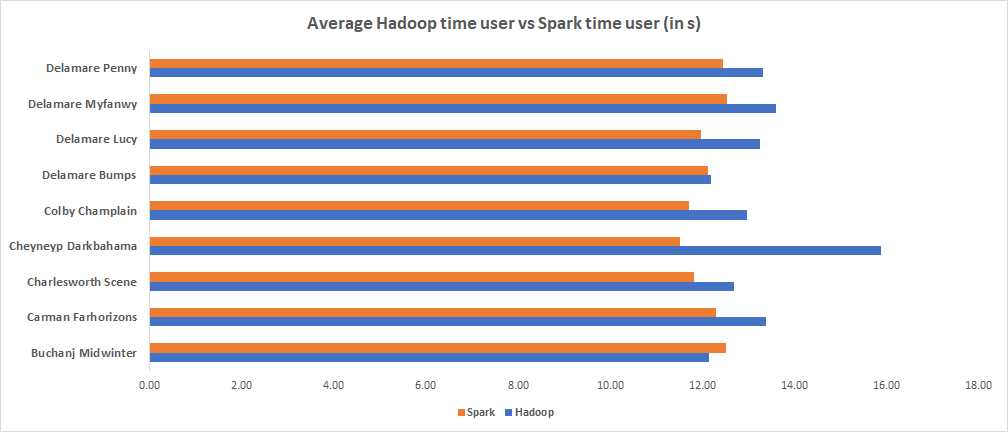
\includegraphics[width=\linewidth]{./images/hadoop-spark.png}
\end{center}

\begin{center}
  \captionof{table}{Comparison between Hadoop and Spark for the 9 texts} \label{tab:regression_analysis_summary}
  \begin{tabular}{|*{3}{c|}}
    \hline
    \textbf{Document} & \textbf{Hadoop time (in s)} & \textbf{Spark time (in s)} \\
    \hline
    buchanj-midwinter-00-t.txt & 12.15 & 12.51 \\
    \hline
    carman-farhorizons-00-t.txt & 13.38 & 12.29 \\
    \hline
    colby-champlain-00-t.txt & 12.97 & 11.71 \\
    \hline
    cheyneyp-darkbahama-00-t.txt & 15.88 & 11.50 \\
    \hline
    delamare-bumps-00-t.txt & 12.18 & 12.12 \\
    \hline
    charlesworth-scene-00-t.txt & 12.7 & 11.81 \\
    \hline
    delamare-lucy-00-t.txt & 13.26 & 11.96 \\
    \hline
    delamare-myfanwy-00-t.txt & 13.59 & 12.53 \\
    \hline
    delamare-penny-00-t.txt & 13.31 & 12.44 \\
    \hline
  \end{tabular}
\end{center}

\subsection{Results}

\paragraph{} We began to experiment with the assumption that Spark would outperform Hadoop due to the fact Apache Spark processes the data in-memory instead of disk after performing a MapReduce. The previous table did not show us what we expected. In fact, we believed Spark would be at least two times faster than Hadoop. When dealing with Big Data, Spark's performance could spike up to three times faster according to Goran Jevtic \cite{1} and according to IBM, Apache Spark can be up to 100 times faster when dealing with smaller workloads \cite{2}. These results could therefore be explained by the fact we aren't dealing with Big Data. Also, the times we obtained might include Spark's warmup phase and therefore is not representative of the actual processing time differences between Hadoop and Spark.

\section{Description of MapReduce jobs to solve the social network problem} \label{sec:MapReduceDescription}
\paragraph{}
For the social network problem, we need an algorithm that recommends friends for each user. More particularly, It needs to find the top 10 of new friends recommendation based on the number of mutual friends. Based on the information given, we can conclude that a MapReduce approach to this problem is very much possible since there is a high amount of data involved (big data) and since this problem is very much parallelizable with the right approach.

\bigskip

Our approach was that for each user we wanted the key-value pair to contain the user as the key and a recommended friend as the value. To achieve this, here is how we separated the map and the reduce part.

\bigskip

\begin{center}
  \begin{minipage}{.7\linewidth}
    \textbf{Note}: The following code runs Hadoop in standalone mode, therefore we only use a single node to execute the program. Performances may vary depending on the user's computer. The average execution time was around one minute.
  \end{minipage}
\end{center}

\subsection{Map}
\paragraph{}
For the map part, the idea was to represent two types of relationships between the users which are a relationship of friendship (already friends) and a relationship of potential friend recommendation. Here we use potential because at this stage we can't know if the two users are already friends or not. This verification will be done during the reduce part. For this problem, the friends of the current user are represented by a friendship relationship since they are already friends. As for the potential friends, they are simply represented by the pairs of permutations between the friends of the current user. As an example, if user 0 has friends {1,2,3}, the potential friends are (1,2) (2,1) (1,3) (3,1) (2,3) (3,2). Since each map process uses as an input one user and it's friend, which are represented by a line of input text file, it's easy to scale up by using, for example, one worker per line of text.

\subsection{Reduce}
\paragraph{}
The reduce part is where most of the work happens in this situation. The idea here is to separate, for the current user, the users that are already friends with him and the users that are recommended as new friends. For the users that are already friends with the user, they are going to be ignored. As for the users that are recommended as new friends, they will be stocked along with the number of mutual friends between them and the current user. The number of mutual friends is given by incrementing everytime there is an occurrence of the recommended user (1 per mutual friend). Finally, the 10 top users with the most mutual friends with the current user will be displayed.

\pagebreak

\section{Algorithm description} \label{sec:MapReduceAlgorithm}

\subsection{Main}
\paragraph{}
The main class is very straightforward. It defines the configuration of the Hadoop Job that will be run. This includes the Mapper class, the Reducer class, the input, the output and more.

\begin{center}
  \captionof{figure}{Main class PeopleYouMayKnow.java}
  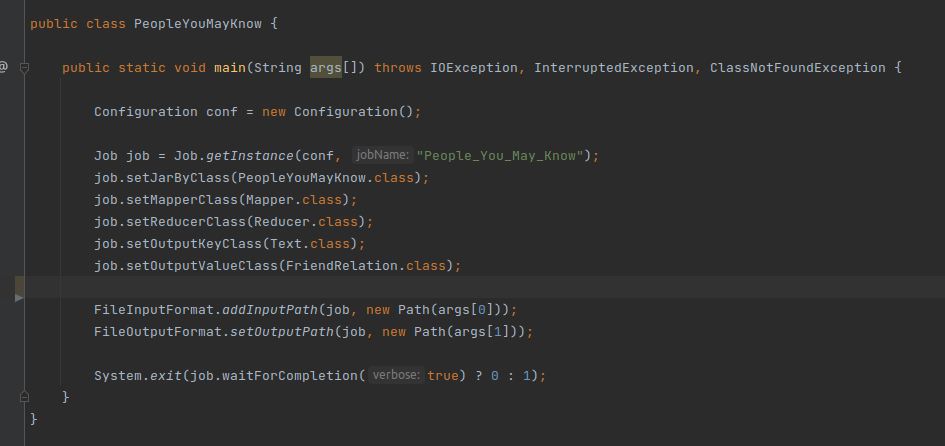
\includegraphics[width=\linewidth]{./images/6-main.png}
\end{center}

\subsection{Map}
\begin{enumerate}
\item The mapper takes the line of input from the input file and separates the current user (key) and it's friends (value).

\item An iteration is done through it's friend list and the program output the current user and his friend with an \textit{already friend} relationship. The output is a key-value pair with the current user as key and a FriendRelation (see below) as the value.

\item After that, the program finds all the \textbf{unique pairs of permutations} between the friends of the current user and output a potential recommended friend for each permutation. The output is then a friend of the current user as a key and a FriendRelation as the value.
\end{enumerate}

\pagebreak

\begin{center}
  \captionof{figure}{Mapper class Mapper.java}
  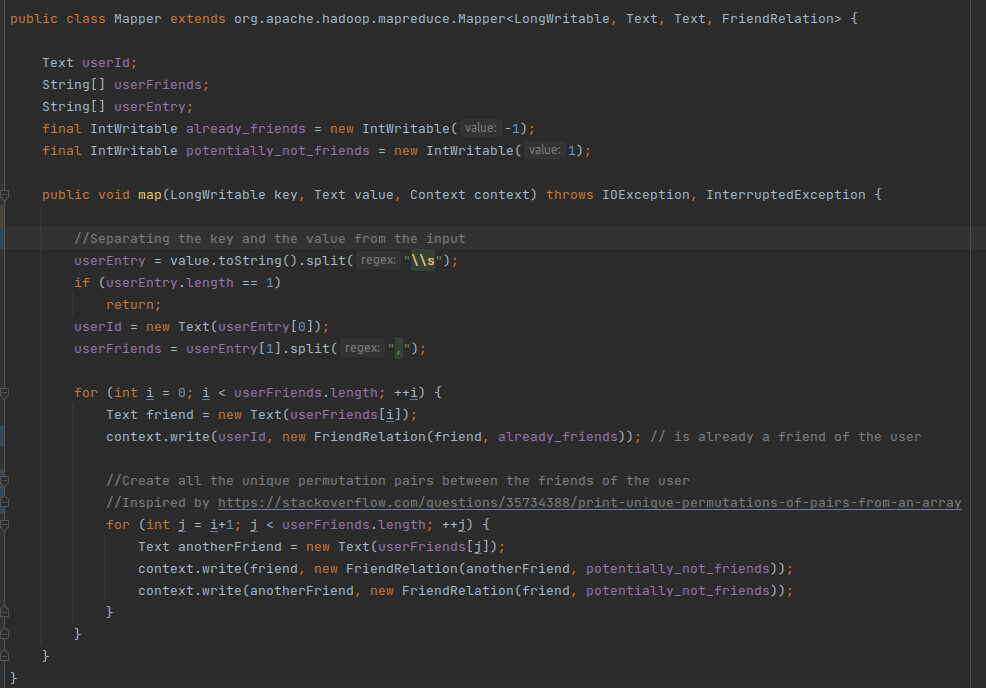
\includegraphics[width=\linewidth]{./images/6-map.png}
\end{center}

\subsection{FriendRelation}
\paragraph{}
This class is used as the output (value of the key-value pair) of the Mapper. It defines a user with it's relationship with the current user (defined in the key of the key-value pair). For example the key-value pair {1, (2, -1)} could be interpreted as \textit{user 1 is already friend with user 2}.

\begin{center}
  \captionof{figure}{FriendRelation class FriendRelation.java}
  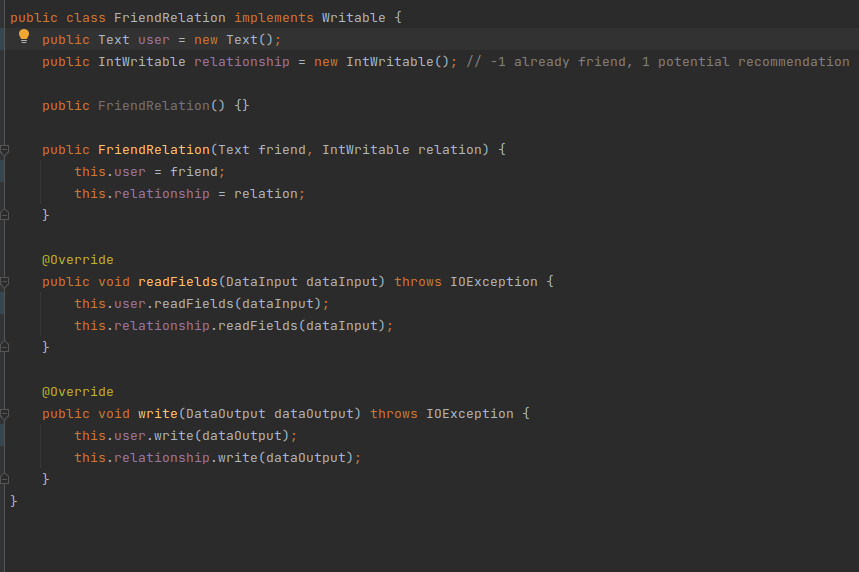
\includegraphics[width=\linewidth]{./images/6-friendrelation.png}
\end{center}

\subsection{Reduce}
\begin{enumerate}
\item The reducer takes all the FriendRelation received from the current user (defined in the key) and iterates over all of them. As mentionned before, if the relationship value in the FriendRelation is -1 then the users are already friends. In that case we put the user in a separate array (currentFriends ArrayList). If it's not -1 then they are potential friends if the other user isn't in the friends array. We then either add the new potential friend in the map (friendsRecommendation HashMap) with a value of 1 or we increment the value by 1. As previously mentionned, this value represents the number of mutual friends between the current user and the other user.

\item The next step is to take the map containing potential friends and to sort it in descending order of the number of mutual friends (value of the map). A TreeSet with a custom comparator was used for that purpose. The custom comparator first compares the value of 2 elements and then, if the values are equal, it compares the user id and prioritizes the smaller one.

\item The last step is to take the first 10 ordered recommended friends by ignoring those who are already friends with the current user. Each recommendation is added to the result that will be outputed.
\end{enumerate}

\pagebreak

\begin{center}
  \captionof{figure}{Reducer class Reducer.java}
  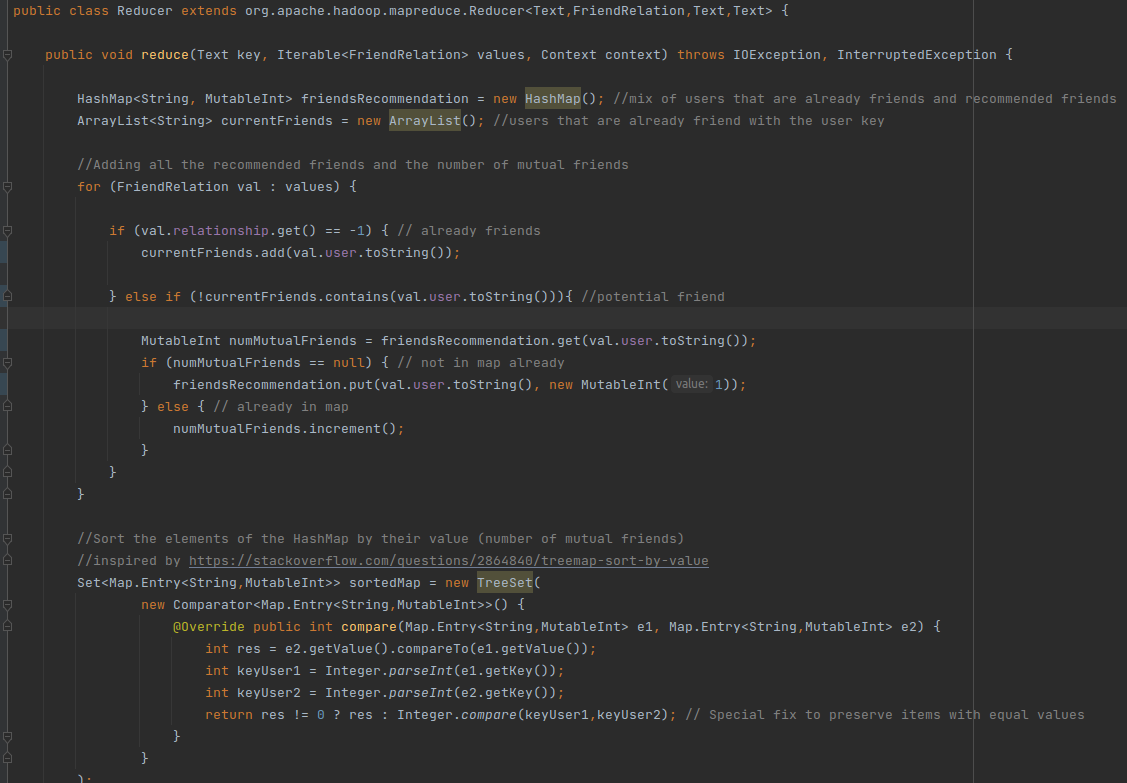
\includegraphics[width=0.9\linewidth]{./images/6-reduce.png}
\end{center}

\begin{center}
  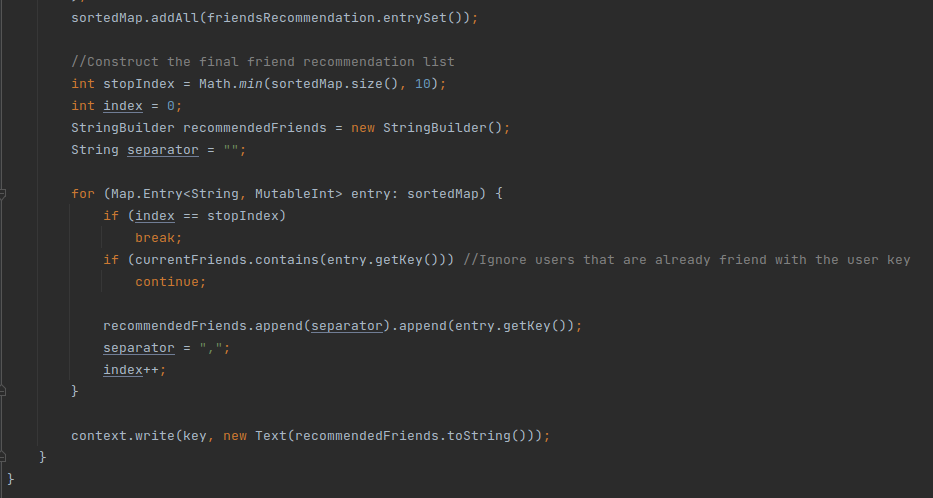
\includegraphics[width=0.9\linewidth]{./images/6-reduce2.png}
\end{center}

\section{Recommendations of connection for some users}

\paragraph{} By looking at the output file provided by the Hadoop MapReduce job, here are the results we found for the requested users:

\bigskip
\begin{center}
  \begin{minipage}{.7\linewidth}
    924  \hspace{0.9cm}  439, 2409, 6995, 11860, 15416, 43748, 45881 \\
    8941 \hspace{0.7cm}  8943, 8944, 8940 \\
    8942 \hspace{0.7cm}  8939, 8940, 8943, 8944 \\
    9019 \hspace{0.7cm}  9022, 317, 9023 \\
    9020 \hspace{0.7cm}  9021, 9016, 9017, 9022, 317, 9023 \\
    9021 \hspace{0.7cm}  9020, 9016, 9017, 9022, 317, 9023 \\
    9022 \hspace{0.7cm}  9019, 9020, 9021, 317, 9016, 9017, 9023 \\
    9990 \hspace{0.7cm}  13134, 13478, 13877, 34299, 34485, 34642, 37941 \\
    9992 \hspace{0.7cm}  9987, 9989, 35667, 9991 \\
    9993 \hspace{0.7cm}  9991, 13134, 13478, 13877, 34299, 34485, 34642, 37941 \\
  \end{minipage}
\end{center}

\section{Instructions to run the code} \label{sec:RunningTheCode}

\subsection{WordCount on Spark}
\begin{enumerate}
\item Install Spark 3.2.0 and Maven
\item Create a new directory (e.g. sparkwordcount) which will include the SparkWordCount.scala program
\item Copy-paste the pom.xml file (available in the git repository) in the \textit{sparkwordcount} directory and generate the application jar by running the following command in that same directory:

  \begin{center} \textit{\$ mvn package} \end{center}

  \textbf{Note}: this will generate a file named \textit{sparkwordcount-0.0.1-SNAPSHOT.jar} in a new directory named \textit{target} (e.g. ./sparkwordcount/target)

\item Launch the SparkWordCount.scala script from its directory (~/tp2/wordcount) by typing the following command:
  \bigskip
  \begin{center}
    \begin{minipage}{.7\linewidth}
      \textit{\$ time spark-submit -{}-class SparkWordCount \textbackslash \\ YOUR\_LINK/target/sparkwordcount-0.0.1-SNAPSHOT.jar \textbackslash \\  YOUR\_LINK/YOUR\_FILE.txt}
    \end{minipage}
  \end{center}
\end{enumerate}

\subsection{Demonstration}

\bigskip The link for the git repo that contains all the code is:
\url{https://github.com/faynz/finalproject-log8415}

\bigskip The link for the youtube demonstration is:

\bigskip \noindent \textbf{The requirements} for this projects are : AWS CLI

\bigskip \noindent To run the code, you simply have to run the bash script named: "launch.sh"

\section{Conclusion} \label{sec:Conclusion}
\paragraph{}
In conclusion, I am pretty disappointed in the outcome of this final project. I wish I had more time to complete the full project and get to learn how to automate website deployment on EC2 instances as well. I will probably look into it for myself.
The project was very benificial, I learned a lot about the available services offered by AWS and the platform itself. It was quite interesting to see how quickly and efficient it is. It allows for very quick updates.

\begin{thebibliography} {}
\bibitem{1} https://medium.com/@kyle.galbraith/how-to-host-a-website-on-s3-without-getting-lost-in-the-sea-e2b82aa6cd83
\bibitem{2} https://docs.aws.amazon.com/codepipeline/latest/userguide/tutorials-s3deploy.html
\bibitem{3} https://docs.aws.amazon.com/prescriptive-guidance/latest/patterns/automate-static-website-deployment-to-amazon-s3.html
\bibitem{4} https://docs.aws.amazon.com/AmazonS3/latest/userguide/HostingWebsiteOnS3Setup.html
\bibitem{5} https://gist.github.com/shortjared/4c1e3fe52bdfa47522cfe5b41e5d6f22
\bibitem{6} https://docs.aws.amazon.com/cli/latest/reference/sts/get-caller-identity.html
\bibitem{7} https://docs.aws.amazon.com/codepipeline/latest/userguide/reference-pipeline-structure.html
\bibitem{8} https://docs.aws.amazon.com/codepipeline/latest/userguide/reference-pipeline-structure.html#reference-action-artifacts
\bibitem{9} https://docs.aws.amazon.com/codepipeline/latest/userguide/appendix-github-oauth.html#action-reference-GitHub
\bibitem{10} https://docs.aws.amazon.com/cli/latest/reference/codepipeline/create-pipeline.html

\end{thebibliography}

\section{Annex} \label{sec:Annex}
Link to the git repository: \\  \url{https://github.com/faynz/finalproject-log8415}
\end{document}

\#+end\textsubscript{export}
\end{document}
